% Chapter 2
\chapter{Theoretical Background, Fundamentals and Preliminary Work}

\lhead{Chapter 2. \emph{Theoretical Background, Fundamentals and Preliminary Work}} % This is for the header on each page - perhaps a shortened title

%----------------------------------------------------------------------------------------
\section{Introduction}

In this section, the main terms and used technologies are discussed. Several positioning principles and their suitability for providing the mobile guide's location context are described. As Swift is a very young language\footnote{Swift 1.0 was released on Sep 9, 2014} and thus merits closer consideration, a subchapter is dedicated to Swift and hot it compares to Scala. As preliminary work for the evaluation of the new proximity technology BLE (Bluetooth Low Energy) Beacons, a Swift-Prototype was implemented and is presented in this chapter, too.

\section{What is Context-Aware Computing?}

The term "context-aware computing" was first used by B. Schilit et. al. 1994 in the paper "Context-Aware Computing Applications" \cite{Schilit94context-awarecomputing}. They introduce this new kind of computing as a "new class of applications that are aware of the context in which they are run. Such context-aware systems adapt according to the location of use, the collection of nearby people, hosts, and accessible devices, as well as to changes to such things over time".

\subsection{Definition of Context}

Schilit defined context by enumeration of examples that are all related to location and proximity.

Dey and Abowd provided a precise universal definition of context in their paper "Towards a Better Understanding of Context and Context-Awareness" published 1999 \cite{Abowd99}: "Context is any information that can be used to characterize the situation of an entity. An entity is a person, place, or object that is considered relevant to the interaction between a user and an application, including the user and applications themselves."

While being precise, this definition is too general to get an idea of which kind of context information an application could use. So the following subchapter provides a wider list of context examples and a categorization.


\subsection{Categories of Context}

There are many different types of context: 

\subsubsection*{Computing Context}

Some examples are network connectivity, communication costs and bandwidth or available resources like printers, displays and input devices.

\subsubsection*{User Context}

\begin{itemize}
\item The user's \emph{identity}, including his age, gender, education, profession, interests. In today's age of social media the user's connections to other people and their identity are important and widely available as well.
\item The \emph{location} is the most obvious kind of user context. It can be subdivided in two different sub types of location: \\
  Logical location, e.g. "at home" or "at work" or slightly different "in a library, restaurant, cinema"\\
  Absolute location, e.g. "47\textdegree40'02.0"N 9\textdegree10'19.7"E" as geographic coordinates on earth or 2nd floor room 205 in the F-Building of HTWG Konstanz.
\item The \emph{emotional state} indicating if the user is happy, angry, worried etc. At which level is the personal stress level?
\item \emph{Fisical state}: Is the user rested or tired?
\item The user's \emph{health state}, determined by measuring some vital parameters (e.g. hearth rate, blood pressure and oxygen saturation). Many  dedicated low-cost hardware items for this kind of measurements were released in 2014 or are announced for this year. 
\item Information about other people or mobile devices nearby forms the \emph{co-location} context.
\item The current \emph{activity}. For example walking, driving a car, riding a bicycle or jogging. Some of this activities need to be further specificated, e.g. jogging to practice sport or jogging for catching a train.
\end{itemize}

\subsubsection*{Time Context}

The time context, such as the current time of the day, the day of the week, the current season or the full date. 

\subsubsection*{Physical Context}

Some examples for environment information are the current temperature, the weather, the intensity of ambient light, the noise level and even traffic condition.

cf. \cite{distributed-cas}


\subsection{Categories of Context-Aware Applications}

Schilit and his co-authors describe the following four categories of context-aware applications:

\begin{itemize}
\item Proximate Selection

Highlighting actions or information based on the current location of the user is called "Proximate Selection". While this user interface technique generally requires a user entering his location manually, context-aware systems default it automatically to the currently sensed location. \\
Nowadays, we encounter this behavior in many smartphone applications like weather forecasts for the current city, searching nearby stores in digital yellow-pages or even when performing online searches on non-portable computers.

\item Automatic Contextual Reconfiguration

"Automatic Contextual Reconfiguration" means loading and activating different system configurations based on the current context of use. For example, loading a different digital whiteboard per room gives the illusion of accessing it as if it was physically mounted in that room. But the considered context information is not limited to the location. Changing the energy plan of a notebook based on the connection status of the A/C power cable or the current battery level are further examples for this category. 

\item Contextual Information and Commands

This category contains systems providing the right piece of information and offering the adequate actions at the right time fitting the current context.

Retrieving information provided as text, audio, picture and video form, fitting to the current location context of the user is obviously a key feature of the museum guide that is developed as part of this master thesis.

\item Context-Triggered Actions

Context-triggered actions are applications that execute a defined action when a specific predefined context-state is reached. In contrast to contextual information and commands, these actions are automatically executed. Combining multiple rules allows designing more complex behaviors.

\end{itemize}




Obviously, nowadays there are many applications that fit in two or more categories. A modern smartphone based navigating system for example offers functions like "Take me to a gas station", displaying a list with the nearest one already preselected (proximate selection). When light conditions change, like when entering a tunnel or when it gets dark, the display is automatically dimmed. The pedestrian mode is an example for two categories: The device senses steps and switches automatically into pedestrian mode considering paths not accessible by car (automatic contextual reconfiguration) and offering commands like "Take me back to my parking lot" (contextual commands).



\subsection{Ubiquitous Computing}

The vision and research field of ubiquitous computing was coined 1991 by Mark Weiser of Xerox PARC in his article "The Computer for the 21st Century" \cite{weiserm1991}. 
Weiser's starts his article with these words:
"The most profound technologies are those that disappear. They weave themselves into the fabric of everyday life until they are indistinguishable from it."

For computers, that means being integrated in common objects of daily usage, supporting humans without demanding their full attention. \\
As an excellent example for a technology that disappeared in the background he uses the vanishing of electric motors. At the beginning, big powerful engines powered a whole fabric, with axles and belts distributing the force to the single machines and workplaces. Later, as motor engineering improved, each machine had its own motor and today several electric motors - miniaturized and bigger ones - are integrated into a single device. Often they work in the background letting us focus on the main task. Already in 1991, at the time of his writing, a typical car had more than 20 integrated motors, nowadays even more. They are used to start the engine, lock and unlock the doors, clean the windshield, open and close the windows, align the rear-view mirrors, adjust the seats by several axis and so on. 

Although Weiser didn't use the term context-awareness, he already recognized the importance of the location context: "We have found two issues of crucial importance: location and scale. Little is more basic to human perception than physical juxtaposition, and so ubiquitous computers must know where they are. [...] If a computer merely knows what room it is in, it can adapt its behavior in significant ways without requiring even a hint of artificial intelligence.".

\section{Sensors Integrated in Mobile Devices}

\subsection{Introduction}

Every type of context information has one or more sensors as direct or indirect source. Thus, context-aware computing is only possible with high quality data provided by a variety of sensors.

\begin{figure}[H]
\centering
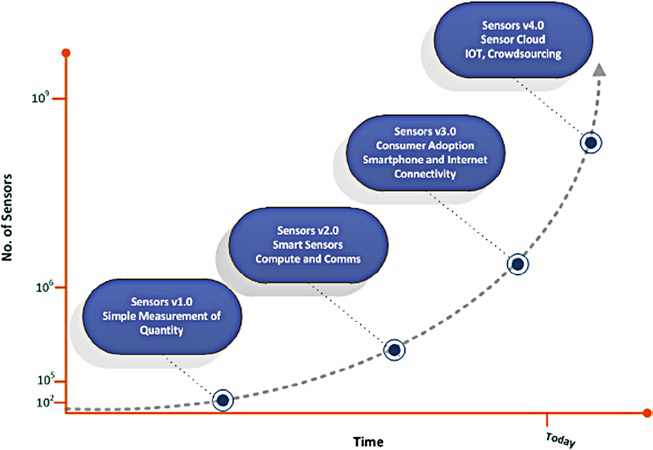
\includegraphics[height=0.20\textheight]{sensors-growth}
\caption{Evolution of sensors \cite[Ch. 1]{sensors-book}}
\end{figure}

According to \cite{sensors-book}, sensors had a enormous growth over the last 30 years and, with accelerating improvement and deployment rates. The authors identify sensors as a technology nexus driven, inter alia, by public healthcare, sports and fitness, pervasive communications and the Internet of Things (IOT). In turn, sensors enable innovation in many sectors, so that one sector benefits of improvements made due the demands of another sector. 

In the next subsections, the major sensors present in mobile devices are presented.

\subsection{Micro-Electro-Mechanical Sensors}

Micro-Electro-Mechanical Sensors (MEMS) are "three-dimensional, miniaturized mechanical and electrical structures, typically ranging from 1 to 100 µm" \cite[Ch. 2]{sensors-book}. They use a movable proof-mass that moves relatively to a frame, electrically measuring the deviation or bending. MEMS are widely used in the automotive industry, where they are part of several systems like the antilock braking system (ABS) or the electronic stability program (ESP). The recent development towards extremely compact, low-cost and power MEMS sensors led to a growing integration in consumer electronics devices like smartphones, tablets and game console controllers. 


\subsubsection*{Accelerometer}

Motion sensing can be separated in five modes: 
\begin{itemize}[noitemsep,nolistsep]
 \item acceleration
 \item vibration (periodic acceleration)
 \item shock (instantaneous acceleration)
 \item tilt (static acceleration)
 \item rotation
\end{itemize}

An accelerometer can measure all of them except rotation.

Combining the measurements for three orthogonal axis, a motion along any arbitrary path in a 3D-space can be reconstructed.

There is one sensed acceleration component always present on Earth: The gravitational acceleration. Near the Earth's surface, this component can be approximated by \(9.81 \frac{m}{s^2}\). The direction of this component allows to deduce the attitude of the device in respect to the ground using the accelerometer.

\subsubsection*{Gyroscope}

MEMS Gyroscopes are able to measure rotatory motion without relying on rotating parts that would require bearings but using a vibrating proof-mass affected by Coriolis forces. 

The following figure shows the three axis of a 3D gyroscope, as it is available in many mobile devices today.

\begin{figure}[H]
\centering
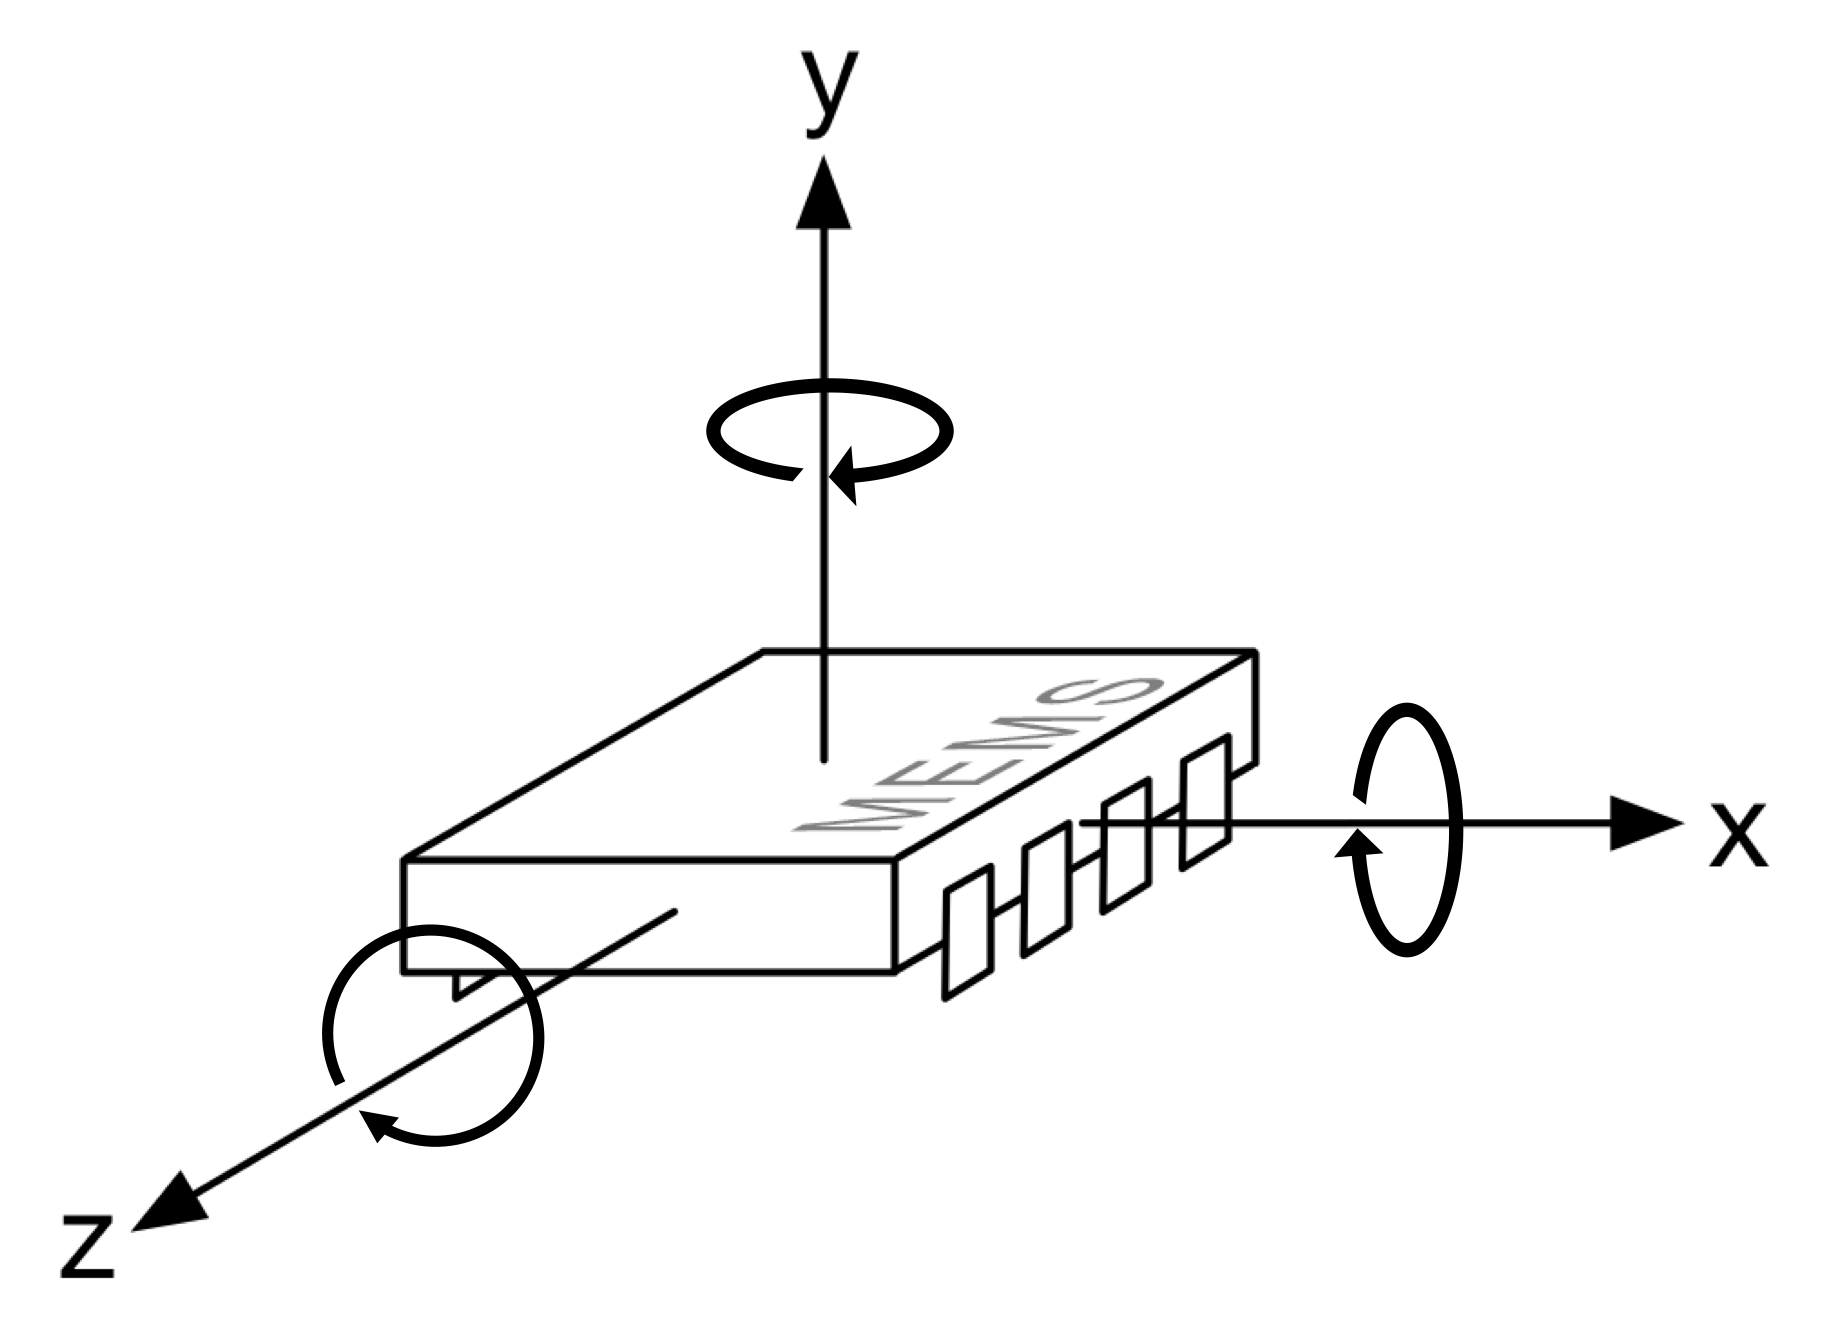
\includegraphics[height=0.20\textheight]{mems-rot}
\caption{The rotation axes of a three dimensional MEMS Gyroscope}
\end{figure}

\subsubsection*{Barometer}

Some of the latest smartphones and tablets are equipped with a MEMS barometer for measuring the air pressure. This information combined with the current weather dependent ground pressure can be used to determine the current altitude or the floor of the building the device is in. 

\subsection{Other Sensors}

\subsubsection*{GPS Sensor}

A GPS Sensor is integrated in many of today's mobile devices. It is a standard part of almost every smartphone and an optional part of many tablets, often bound to a cellular connectivity module. For details on the accuracy, see \ref{gps-prec}.

\subsubsection*{Magnetometer}

The magnetometer acts mainly as digital compass.

\subsubsection*{Proximity Sensor}

The proximity sensor typically measures the distance of the device's front to the next object. It is used to turn off the display when holding a mobile phone at the ear or to determine if the phone is inside a pocket.

\subsubsection*{Light Sensor}

The light sensor measures the intensity of the light. It is primarily used to adapt the screen brightness to the ambient light.

\subsection{Conclusion}

Sensors are evolving rapidly and there are already a broad spectrum integrated in common consumer products like smartphones and tablets. The better the quality of the sensors and the variety of measurable quantities, the more precise and sophisticated can context-sensitive software become.
Sensor data from different sensors is often combined. For example, a magnetometer and gyroscope can be combined to a fast reacting improved electronic compass without drifting. %TODO Quelle

In the next section addresses different localization techniques and discusses how they can be used for the guide system to be designed.  

\section{Localization Techniques}

\subsection{Introduction}

As already emphasized, the location context is very important for many context-aware applications and especially for the visitor guide that will be designed and implemented during this work. 
Therefore a short overview of available positioning techniques and their classification is provided and their applicability to this work discussed. 

\subsection{Classification}

According to (\cite{positioning}, cited by \cite[Ch. 1.1]{ellipsoid}) there are two main categories of positioning techniques, that can be further split up into seven different subcategories.

\subsubsection{Techniques Using Relative Measurements}

This techniques are also known as dead reckoning (DR), and they all need an initial position estimate.

\subsubsection*{Odometry}

By measuring the wheel rotations and the angle of the steer axis, the position is estimated. Due to wheel slippage and measurement errors, the position tends to drift away over time.

\subsubsection*{Inertial Navigation}

Using only inertial sensors (gyroscopes and accelerometers) to measure rotation rates and acceleration forces, the new heading can be estimated integrating the gyroscope data once and the new position integrating the acceleration data twice over time. Pure inertial navigation systems are self-contained and don't need external references.%TODO2 IMAGE

Measurement and (numerical) integration errors accumulate very fast, especially for the position due to the double integration, requiring high precision sensors for decent results. With low cost sensors, as they are used today in many mobile devices, the position error grows unbound already after a very short period of time.

\subsubsection{Techniques Using Absolute Measurements}

\subsubsection*{Electronic Compasses}

Electronic compasses are not a stand-alone positioning solution, but they provide heading measurement to the magnetic north pole. When the declination  angle (the angle between magnetic and geographic north pole) is known for a specific place on Earth, the actual north heading can be calculated. However, local magnetic fields can have a huge impact on the measurements. Near power lines and metallic structures like the structural steel beams in buildings have an impact on the measurement.

\subsubsection*{Active Beacons}

If the environment is already known and beacons are mounted on defined positions, the position of a moving platform can be determined either by triangulation, trilateration or fingerprinting algorithms. Triangulation involves measuring the angles at which at least two beacons are seen. For a trilateration algorithm, the position is calculated by measuring the distance to the beacons. Fingerprinting needs the preliminary creation of a database of measurements at different positions. The position is then estimated by choosing the position-measurement pair out of the database that best fits the current measurement.

\subsubsection*{Global Navigation Satellite Systems}

Abbreviated GNSS, the most well-known example is GPS (Global Positioning System). The receiver can calculate it's position by performing a trilateration. The input is the difference of the travel time of the different satellite's signals and their current location included in the signal. GPS provides good absolute localization for outdoor environments. Indoor, the signal is either very poor or not available at all. %TODO2 Define good with source

\label{gps-prec}
The GPS accuracy of current consumer tablets and smartphones was examined in \cite{gps-precision}. The authors compared measurements from six different smartphones and tablets with reference coordinates, both with static and moving devices. The average error in static measurements ranged from 2.18 to 4.18 meters with standard deviations of 0.82 to 2.17 meters. In case of moving devices, two devices had better results and four showed higher errors with average deviations ranging from 1.76 to 5.15 and standard deviations of 0.61 to 2.50 meters (ignoring one statistical outlier with an average error of 15.08 meters).


\subsubsection*{Landmark Navigation}

Similar to active beacons, this technique requires a well known environment with distinct natural or artificial fixed objects, whose position, exact size and shape must be well known in advance. Most landmark navigation systems are based on computer vision.

\subsubsection*{Map-Based Positioning}

With this technique, a local map is created using sensors like cameras and laser range finders and compared to global pre-stored map, e.g. a CAD model of the environment. If a part of the global map matches the local map, the position can be determined. 

\subsection{Discussion}

A robust and computationally not very expensive technique is needed to efficiently use the limited battery power of mobile devices. Furthermore, that technique must be satisfied by the sensors currently available in common mobile devices alone.

GPS is a good choice for outdoor positioning, being technically mature and widely available on mobile devices. The substantial power drain often associated to the activation of GPS in mobile devices is mostly caused by CPU-intensive navigation software and an active screen rather than the actual sensor.

For indoor navigation, Map-based positioning and landmark navigation can be clearly excluded due to their demands.

Although inertial navigation combined with human odometry is very promising, they require the inertial measurement unit (IMU) to bee foot mounted. The reason is being able to re-calibrate the system and thus the drifting (set the current speed to zero), every time one foot rests on the ground while walking \cite{footslam}. The authors are confident, that "projecting the improvements in microelectromechanical system (MEMS)-based inertial sensors to the next ten or even 20 years, it is foreseeable that FootSLAM will no longer require the inertial sensors to be mounted on the foot." Only then will the sensor quality probably be high enough to provide a position estimate with an arbitrarily hold smartphone comparable to the position estimate quality achieved today with a foot mounted IMU. 

So this technique is currently not suitable for providing the location for the guide, although sensing the steps and thus the pace of the visitor is a goal to keep in mind.

The most promising technique for inexpensive indoor location are iBeacons (see Ch. \ref{ibeacons}), that fall into the category of active beacons. If the quality of the distance measurement has a limited error, a trilateration can provide the position when signals from two or more iBeacons are received. To determine the capabilities of iBeacons, a prototype will be implemented and described in Chapter \ref{prototype}.
 

% Outdoor GPS aided by beacons, Indoor Trilateration with iBeacons, Fallback Some sort of Proximity

\section{Bluetooth Low Energy Beacons - iBeacons}

\label{ibeacons}

\subsection{What is an iBeacon?}

On Mid 2013, Apple introduced iBeacons as new technology for adding location awareness to applications. iBeacons are little devices containig a power cell and a small logic board with a Bluetooth Low Energy (BLE) transmitter. BLE was introduced with Bluetooth 4.0 for applications with very contained power requirements that can be satisfied with 1 Mbps data transfer rates, co-existing with standard Bluetooth \cite{ble}.

iBeacon devices broadcast BLE advertisement packets at an configurable time interval, mostly between 100 ms and 1 s, containing, in essence, a fixed preamble identifying the data as iBeacon advertisement, a set of three configurable device specific numbers and the measured RSSI (Received Signal Strength Indication) in dBm at 1m. The latter value is needed as reference for calculating a distance estimation using the current RSSI measured by the receiving device as input.

Based on the configured advertisement interval and the broadcasting power, that influences the distance until which the beacon ca be detected, the battery is expected to last for up to two years.

Apple provides only the specification and an API, but does not manufacture the devices itself. Instead, third-party supplies, among these a number of start-ups, began to ship iBeacons in 2014. For this thesis, different devices were ordered from estimote (New York, USA), kontakt.io (Kraków, Poland), BEACONinside (Berlin, Germany) and Accent Advanced Systems (Barcelona, Spain). This avoids the risk of concentrating on features or flaws of a specific device brand.

\subsection{The iBeacon Prototype}

\label{prototype}

\subsubsection{Design and Implementation}

The main screen of the prototype provides an overview of all iBeacons in range. %TODO motivation, explanation

\begin{figure}[H]
\centering
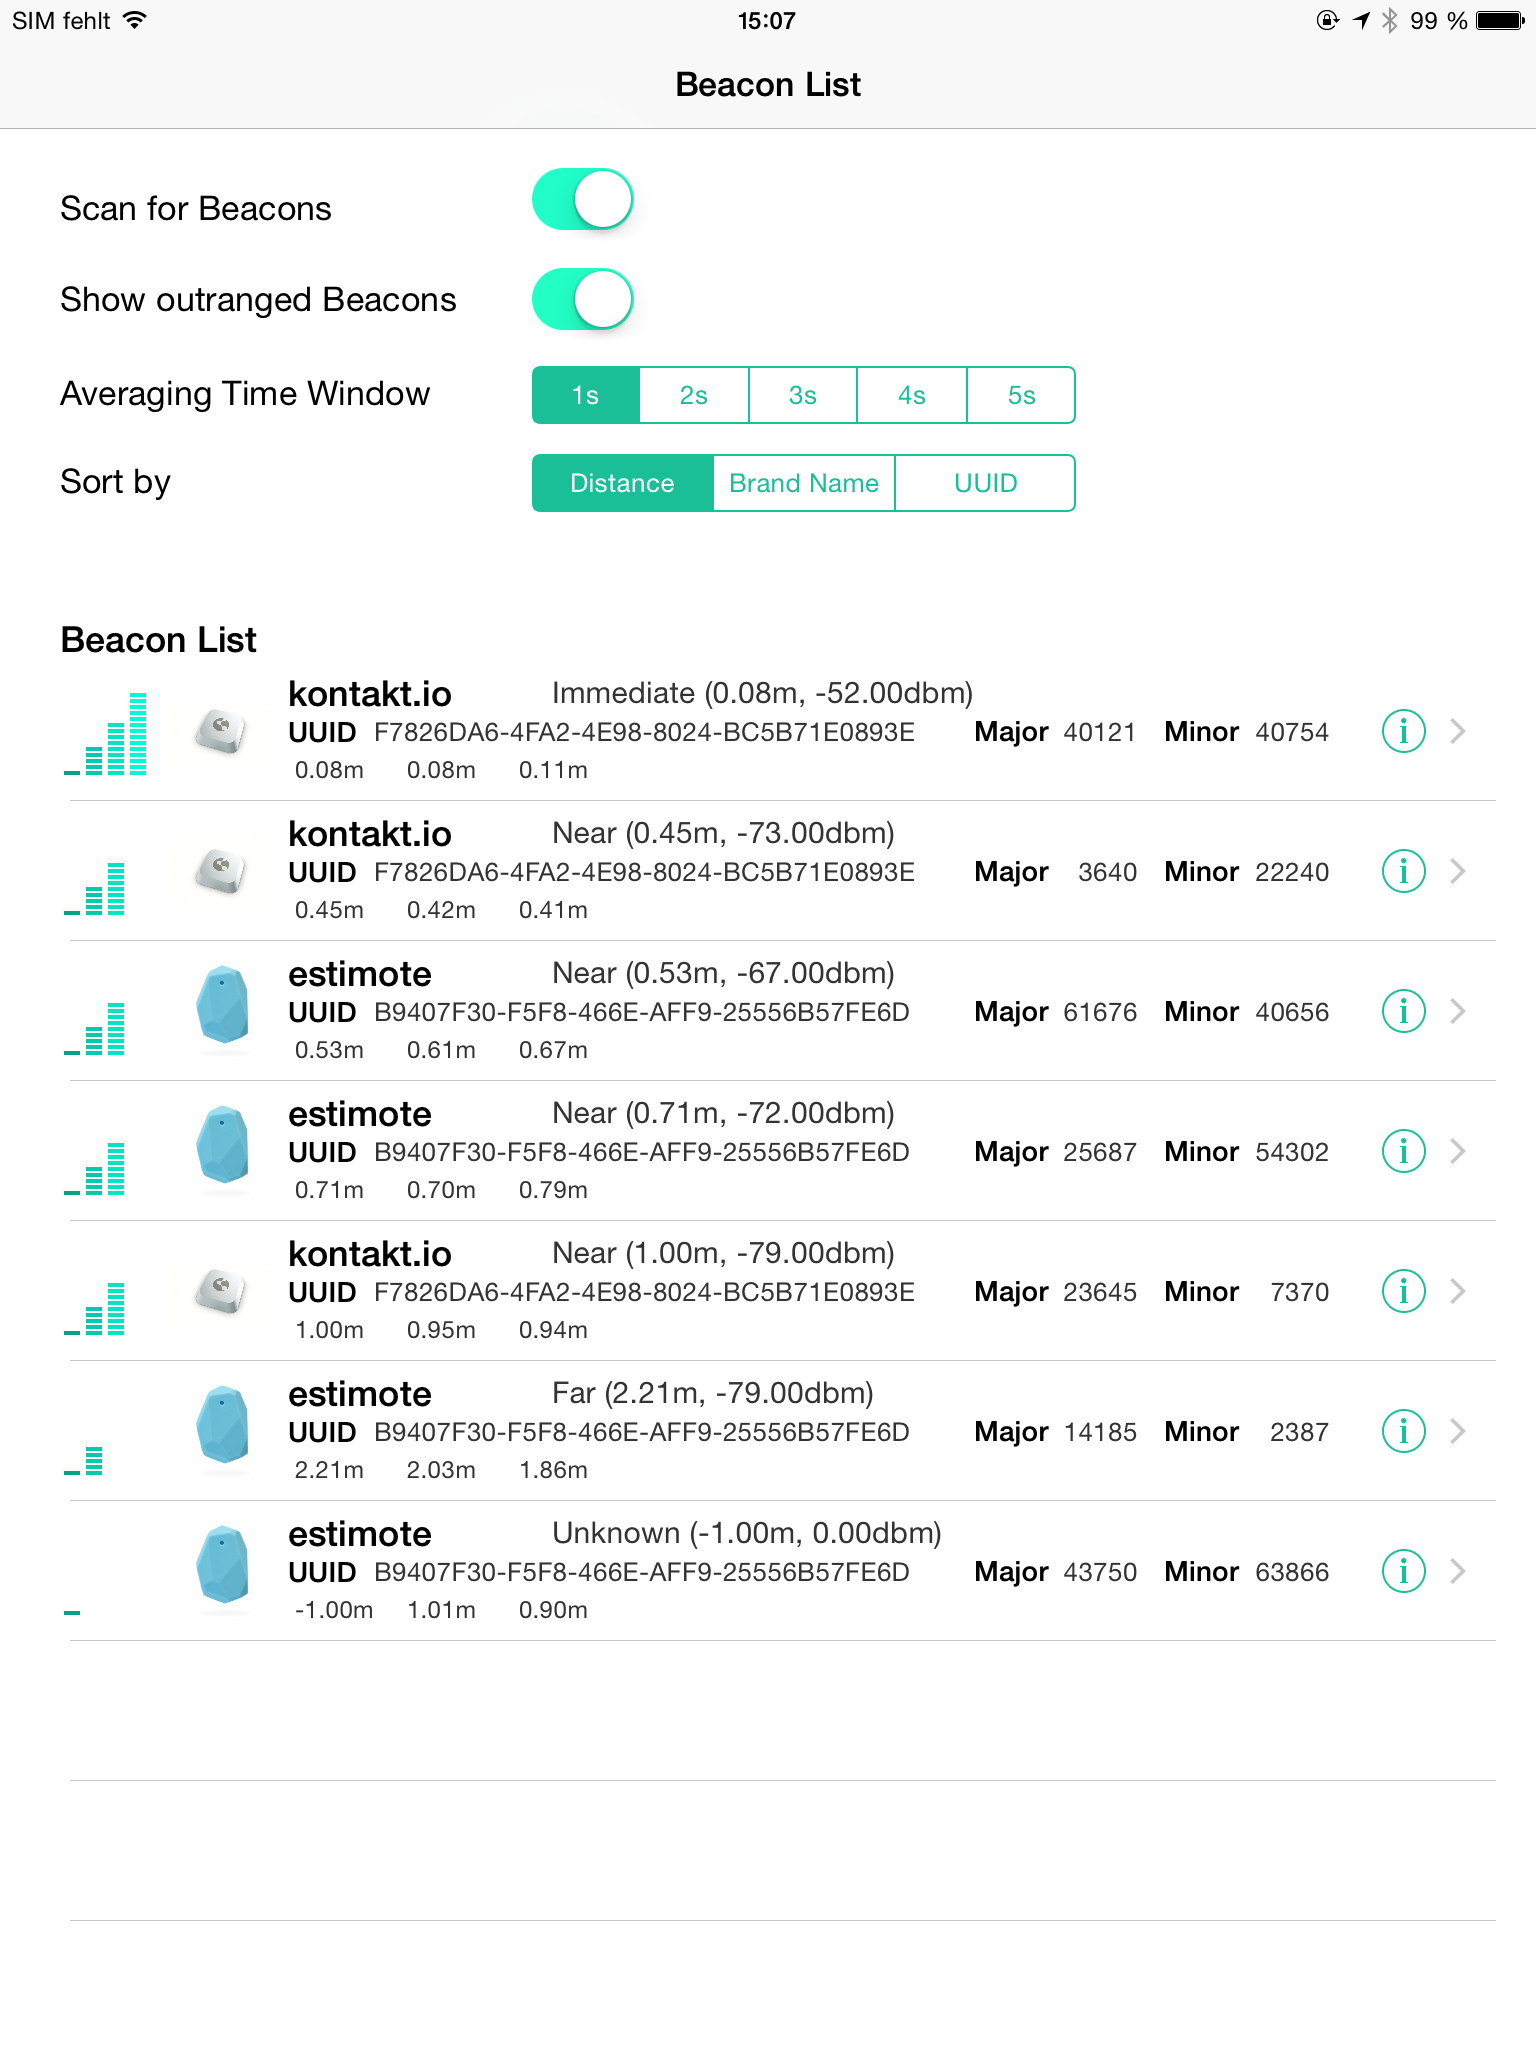
\includegraphics[height=0.40\textheight]{proto1}
\caption{The main screen of the iBeacon prototype}
\end{figure}

After selecting a beacon in the list, the beacon detail view opens showing the details and the single measurements for that beacon on the first screen and some statistics on the second screen.

\begin{figure}[H]
\centering
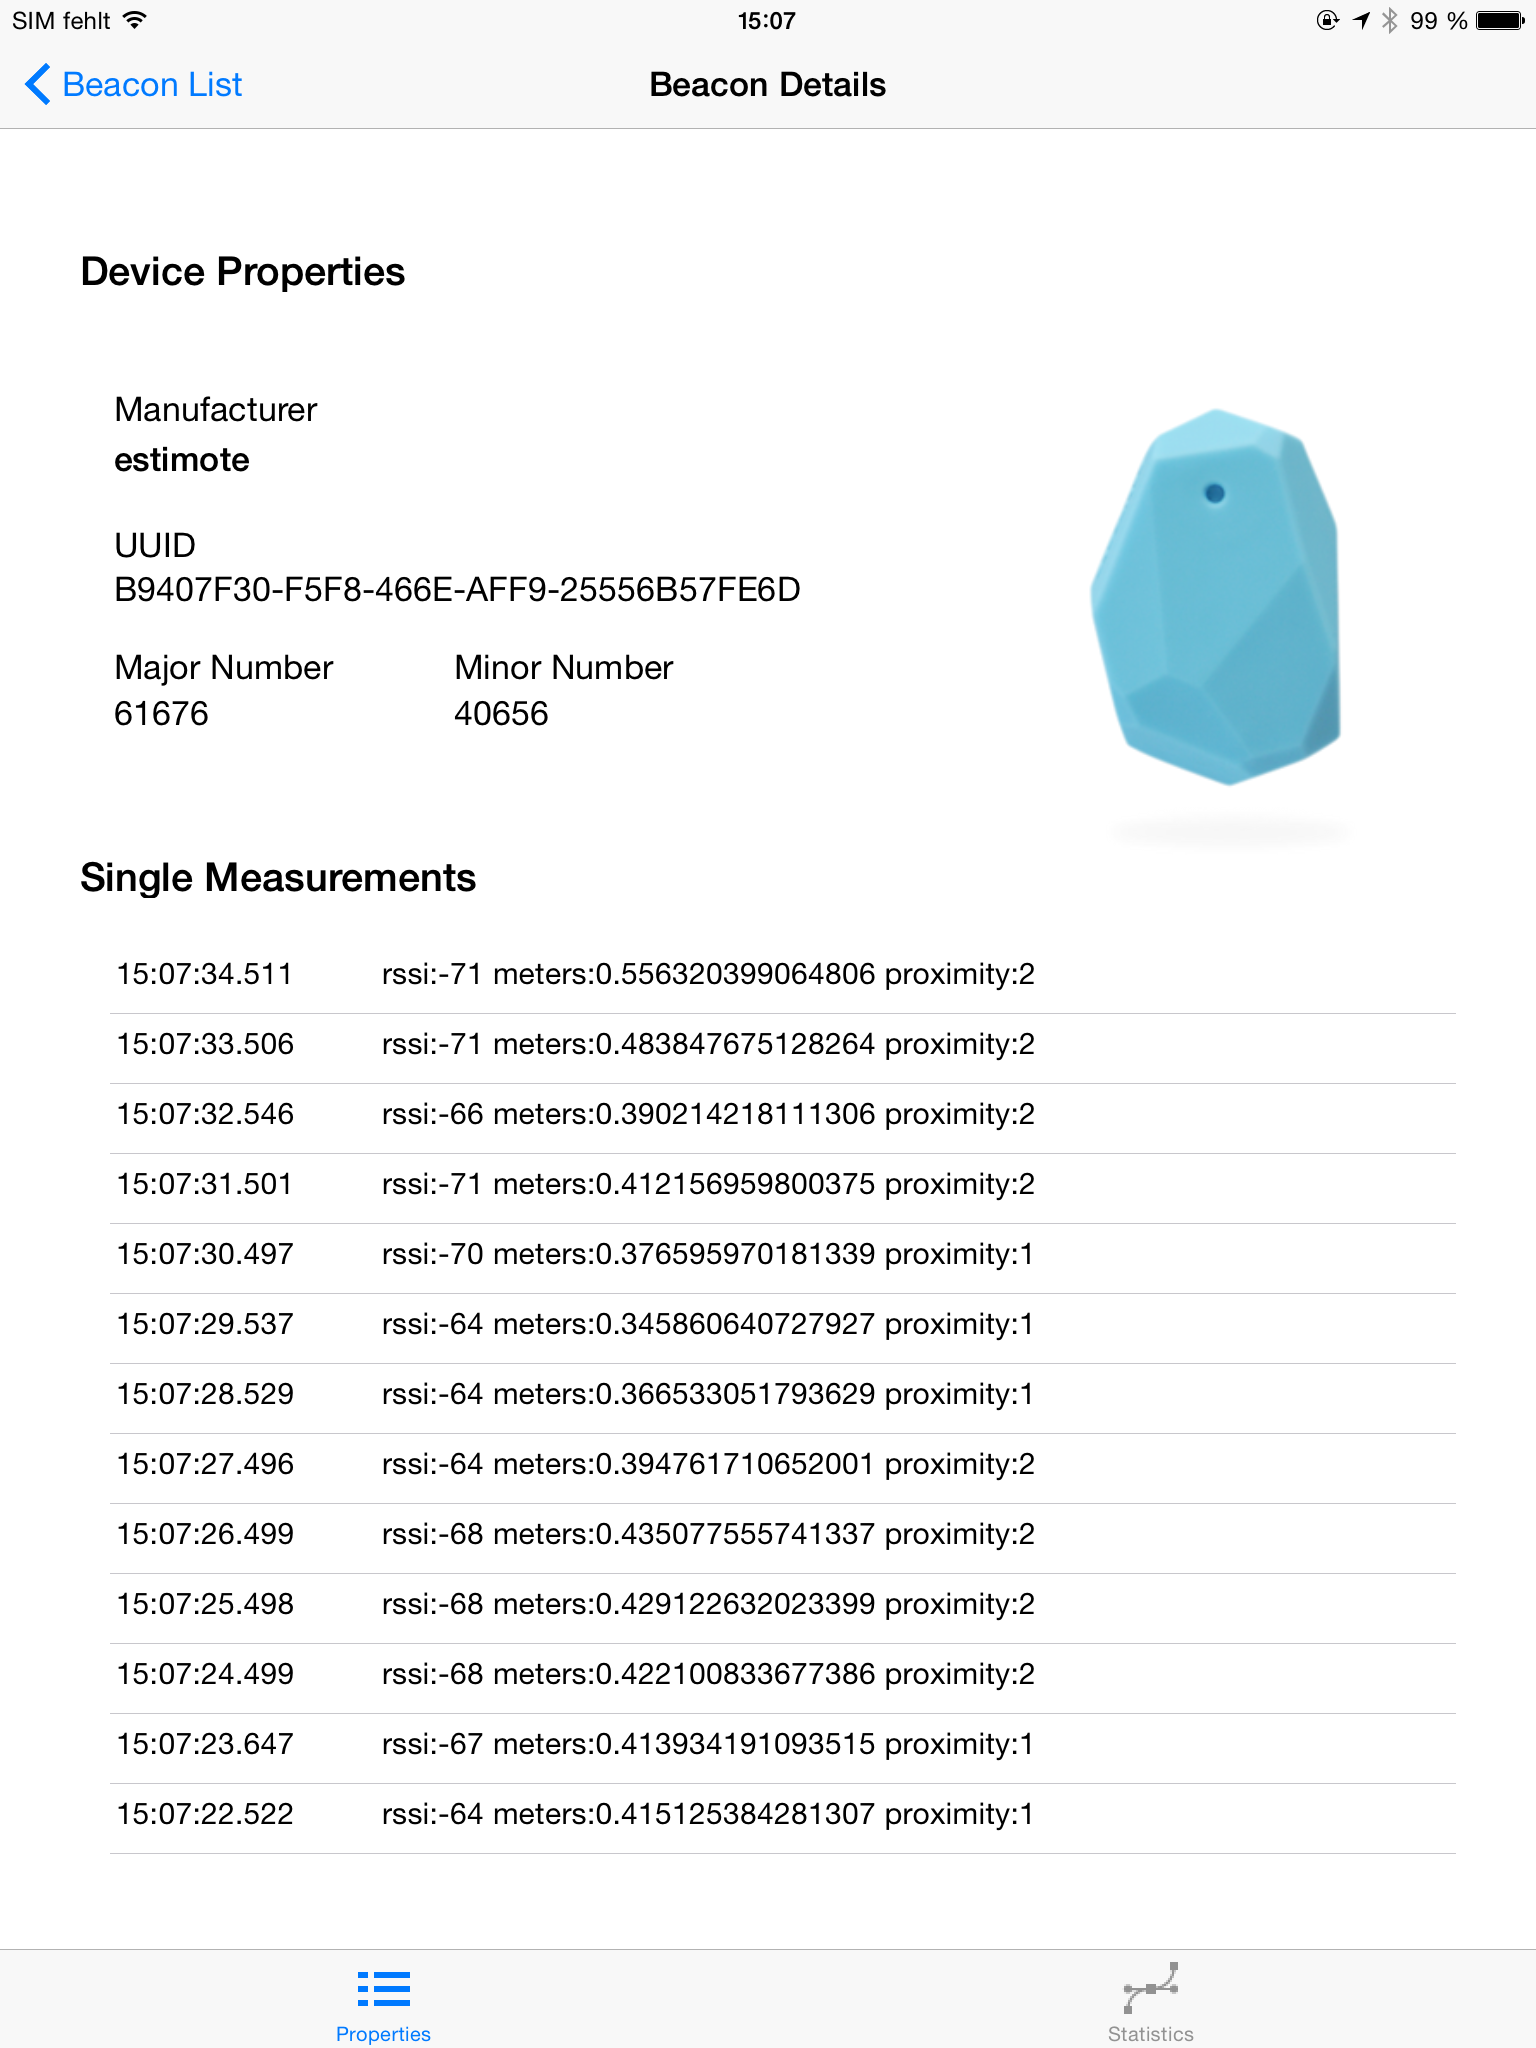
\includegraphics[height=0.40\textheight]{proto2}
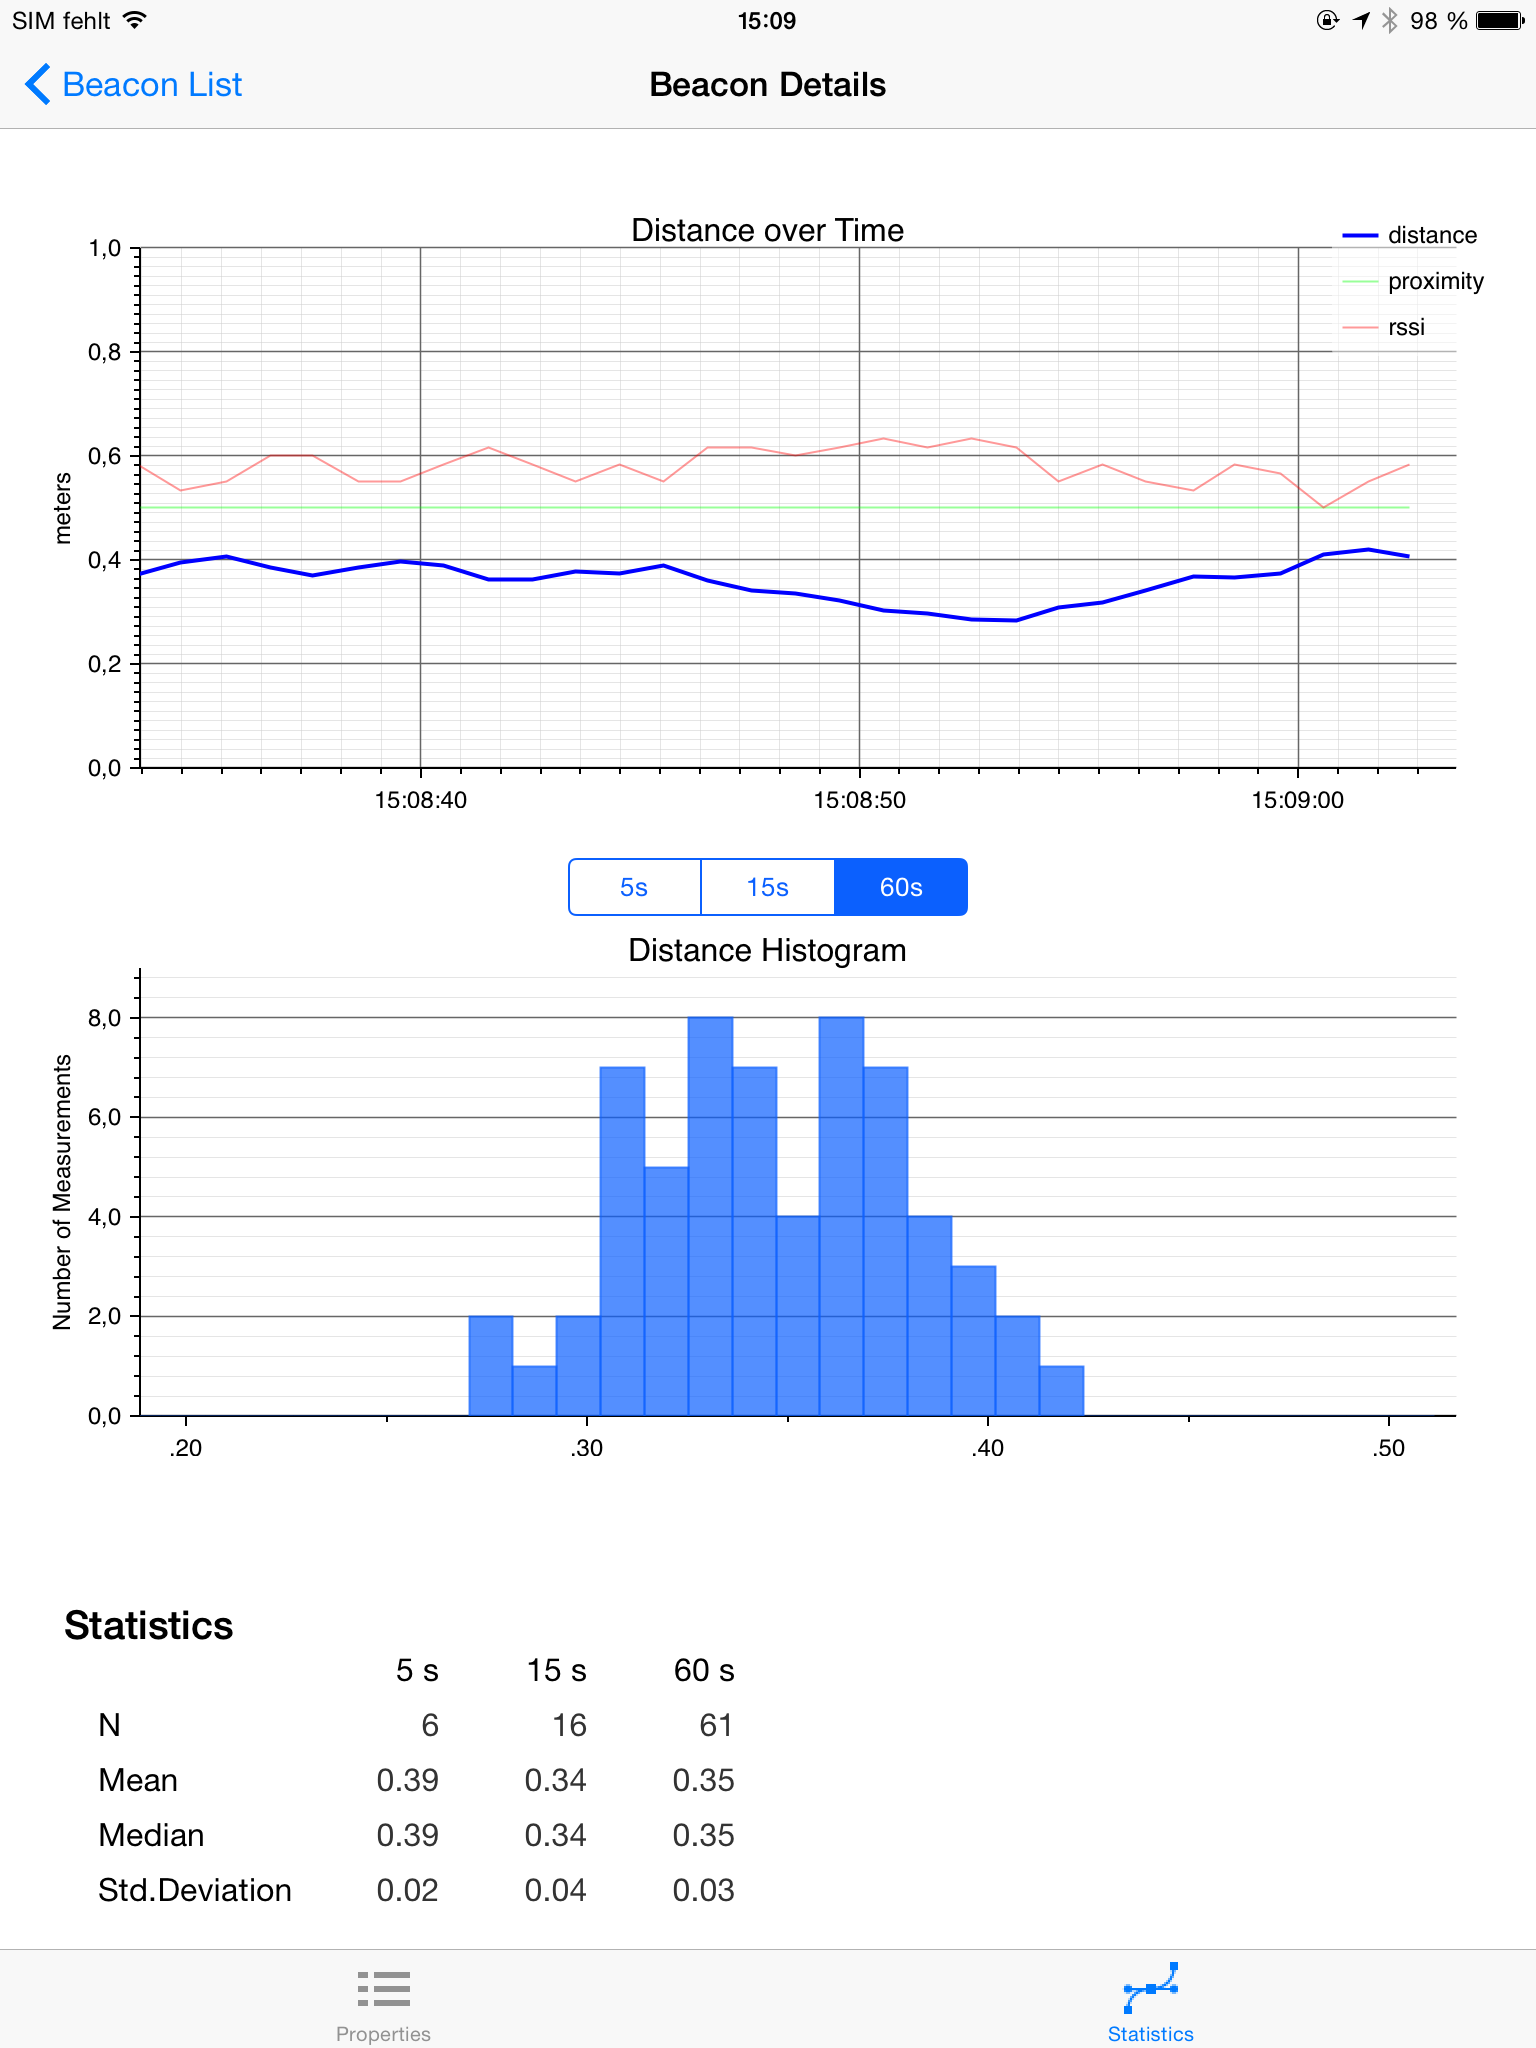
\includegraphics[height=0.40\textheight]{proto3}
\caption{The iBeacon detail screens, including statistics}
\end{figure}

\subsubsection{Measurements and Insights}




\section{Geographic Coordinates}

\subsection{Introduction}

Since we need to work with GPS data on the mobile front end and model outdoor sites like parks on the back end, it is fundamental to understand how the geographic coordinate system works and what kind of problems we may encounter.

\subsection{Standards}

There are many different systems for specifying a precise point on the Earth's surface and describing them all would go far beyond this thesis. The main problem is that the world has a complex shape. Even ignoring tides and winds the sea level does not fit an ellipsoid due to gravity anomalies over the Earth's surface. The surface that most closely approximates sea level is the geoid. 

But for performance and storage reasons an ellipsoid is used in many applications including GPS. One widely used standard is the WGS (World Geodetic System) defining a coordinate system and an ellipsoid. The most recent revision is WGS84, which is exactly what GPS uses and what is used in this work. The ellipsoid can be 106 meters above and 85 meters below the geoid (cf. \cite{geoid}). The following diagram shows the difference in meters between the geoid and the ellipsoid.

\begin{figure}[H]
\centering
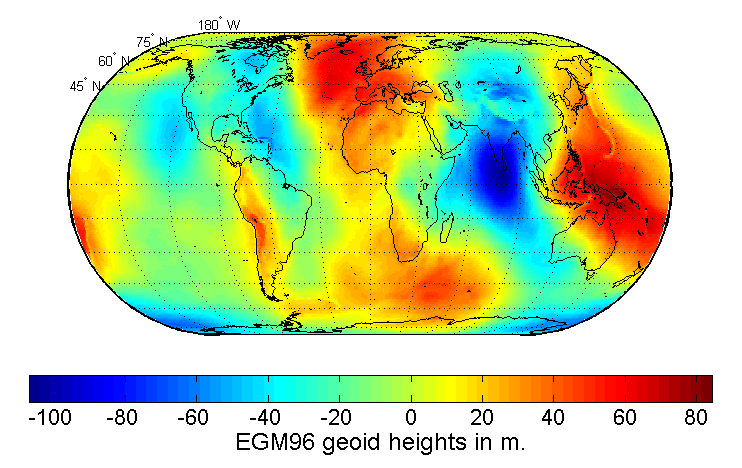
\includegraphics[height=0.22\textheight]{earths_geoidII}
\caption{Difference in meters between the geoid and the ellipsoid \cite{nasageoid}}
\end{figure}

The city of Konstanz, for example, is 46.62 meters above the ellipsoid.

\subsection{WGS84 Coordinates}

A specific point on Earth's surface is defined by a Cartesian coordinate pair consisting of the latitude, that specifies the north-south position and the longitude for the east-west position. 

The latitude is defined to be 0° at the equator and goes up to +90° at the geographic North Pole and down to -90° at the South Pole. The longitude, lacking a natural zero point, is measured relatively to the prime meridian, where the longitude is defined to be 0°. The prime meridian of WGS84 is the line of longitude on the geoid starting/ending at the geographic North/South Pole and passing trough a well defined point 102 meters to the east of the Royal Observatory, Greenwich, London. Eastwards the longitude goes up to 180°, to the west it goes down to -180°, meeting at the same meridian - the one opposite to the prime meridian. 

%\begin{figure}[H]
%\centering
%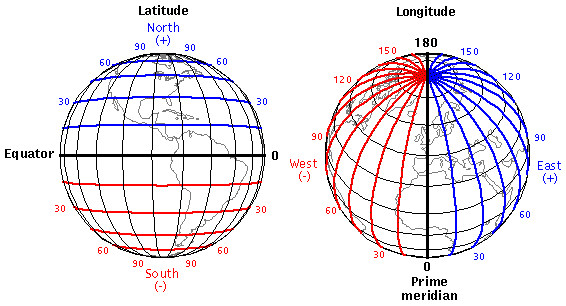
\includegraphics[height=0.15\textheight]{latitude_longitude}
%\caption{Latitude and Longitude }
%\end{figure}
%Source: http://www.nma.gov.au/collections/collection_interactives/european_voyages/european_voyages_to_the_australian_continent/navigation/solving_the_longitude_puzzle

For this work, longitude and latitude are represented by decimal fractions.

The maximum resolution using 6 fractional digits depends on the position on Earth, more specific on the latitude, because all meridians converge at the poles. For the WGS84 ellipsoid, the formula 

\[R_{\phi} = \frac{a \cos\phi}{(1-e^{2}\sin^{2}\phi )^{1/2}}\]

can be used to calculate the radius of the circle of latitude at a given latitude \(\phi\) \cite[cf.][Ch. 2.4]{ellipsoid}. 

The length of one degree of the circumference of that circle of latitude is then calculated with

\[\delta_{\phi}^{1} = \frac{2\pi}{360} * R_{\phi}\]

Solving with latitude \(\phi = 47,6°\) for Konstanz, equatorial radius \(a = 6,378,137.0 m\) and eccentricity \(e = 0,08181919\) as defined in WGS84, the solution is 75.200 km.

So in Konstanz, 0,000001 degree of longitude corresponds to 7,52 cm. The biggest distance, and thus the lowest resolution, is on the equator, where it amounts to 11,13 cm.

The distance of 0,000001 degree of latitude is almost constant at about 11,1 cm. %TODO2 More precise computation

\subsection{Using different Mapping Providers}

One of the most well-known provider for maps is Google Maps, offering a web interface and an API for the integration in own web applications. For iOS development, the native solution is the Apple Map Kit framework, that uses the own Apple Maps service\footnote{Until iOS 5.1, Apple used the Google Maps service and the decided to start it's own competing product}.
%TODO2 Source + apple maps had a bad start

The maps images at the closer zoom levels are in most cases taken by a camera mounted on a plane. This camera often does not look perpendicular to the ground but with a gentle angle, so that you can see the building facades. %TODO Source
While this results in a nice isometric-like perspective, it introduces a problem one has to be aware of: Higher parts of the image like higher floors or small hills appear shifted to a certain direction. 

An example: To check the consistency of Google and Apple maps, I initially used the roof window of the office in which the biggest part of this thesis was written. The coordinates of this window on both maps showed a notable discrepancy of several meters. The cause is the different camera angle of the two pictures. 

\begin{figure}[H]
\centering
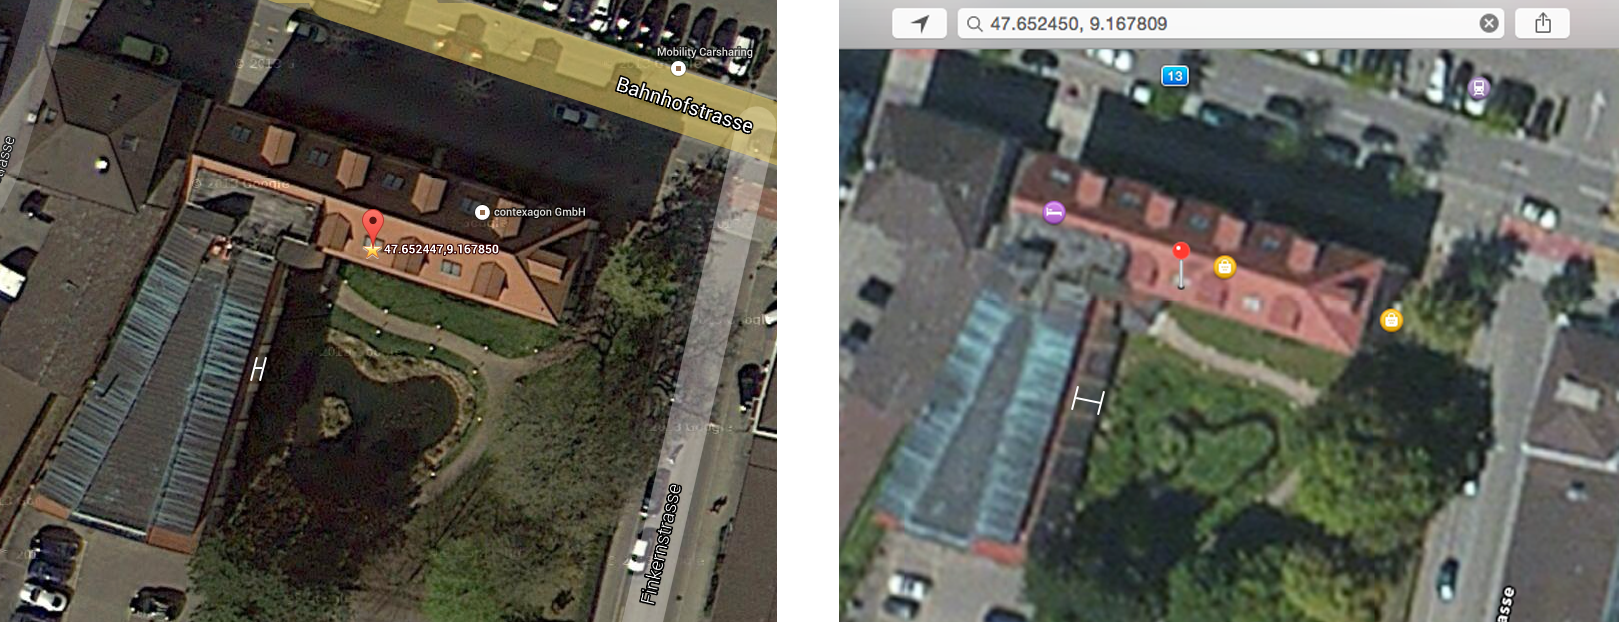
\includegraphics[height=0.22\textheight]{google-apple-maps}
\caption{View angle error on Google (left) and Apple (right) maps}
\end{figure}

This results in a latitude shift from Google to Apple Maps of \(+3 * 10^{-6}\) degrees and a longitude shift of \(-4,1 * 10^{-5}\) degrees. Using the results of the previous section translates in a deviation to the nord of 0,33 m and a considerable deviation to the west of 3,08 meters.

To exclude this view inclination error and get the pure ground coordinate discrepancy of the two mapping solutions, the coordinates of a small distinctive fixed ground object (one of the white lighting poles on the borders of the path in the park) are measured in both mapping solutions.

The measured pure deviation amounts to not negligible \(-1,4 * 10^{-5}\) degrees of longitude or 1,05 meters.

It is important to keep in mind all this different kinds of errors discussed in this section during development and testing of the guide, to avoid searching for errors at the wrong place.


\section{Swift}

\subsection{What is Swift?}

Swift is a modern programming language released by Apple in 2014. In \cite{swift-book} Apple introduces Swift as "a new programming language for iOS and OS X that builds on the best of C and Objective-C, without the constraints of C compatibility".

Since Swift is a cutting-edge language, this section is dedicated more attention as one would normally do for a implementation language inside a thesis. 

Developers already familiar with the well designed functional programming language Scala will recognize several concepts. It has a concise Syntax avoiding big parts of boilerplate code and syntactic noise, supports functional programming and is statically typed.

The following section is an overview comparison of Scala and Swift features, created during the familiarization with Swift for this thesis. Language features marked will a * will be discussed separately in section \ref{majorDiffs}.

\subsection{Comparison Scala and Swift}

\newcommand{\yes}{yes}

\begin{longtable}{|P{5.5cm}|P{4cm}|P{4cm}|}

\hline \textbf{Language Feature} & \textbf{Scala} & \textbf{Swift} \endhead
\hline Type inference & \yes & \yes \\
\hline Line end separates commands (no need for semicolon) & \yes & \yes\\
\hline Implicit type conversions * & \yes & no \\
\hline Default access levels (access level has to be only provided if it differs from default) & \yes & \yes \\
\hline Functions are first class types\footnote{Functions can be passed to functions, returned from functions, created at runtime and assigned to variables} & \yes & \yes \\
\hline Closures & \yes & \yes \\
\hline Curried functions & \yes & \yes \\
\hline Operator functions & \yes & \yes \\
\hline Named parameters * & \yes & \yes As fixed part of the method's signature \\
\hline Optionals * & via \smalltt{Option[T]} class & widely used, dedicated Syntax\\
\hline Switch with pattern matching & \yes & \yes \\
\hline String interpolation & \yes \newline \smalltt{"Hello \$nameVar"} & \yes \newline \smalltt{"Hello \textbackslash(nameVar)"} \\
\hline Keyword for variable definition & var radius = 1 & var radius = 1 \\
\hline Keyword for constant definition & val pi = 3.14 & let pi = 3.14 \\
\hline Array literal & \smalltt{Array(1,2,3)} & \smalltt{[1,2,3]} \\
\hline Map literal & \smalltt{Map(1->"a", 2->"b")} & \smalltt{[1:"a", 2:"b"]} \footnote{Maps are called dictionaries in Swift} \\
\hline If condition must be boolean & \yes & \yes \\
\hline Tuples & \yes, but without named elements & \yes\\
\hline Ranges & \smalltt{for i <- 0 to 4} \newline \smalltt{0 until 4} & \smalltt{for i in 0...4} \newline \smalltt{0..<4}\\
\hline Constructor & def this() & init() \\
\hline Extended getter/setter concept * & \yes, no observers & \yes, very flexible concept including observers (willSet() didSet() events) \\
\hline Interfaces & trait & protocol \\
\hline Extension of existing types & \yes & \yes \\
\hline Struct & no & \yes \\
\hline Enum & via extending the Enumeration class & \yes, dedicated keyword \\
\hline "Any" Type & Any, AnyVal, AnyRef & Any (instance of any type, even function types) \newline AnyObject (instance of any class type) \\
\hline Qeury an instance of a type by a key in brackets, like arrays or maps & obj(index) calls obj.apply method\newline obj(index) = newValue calls obj.update(0, newValue) & \smalltt{subscript(i:T) -> T2 \{ \newline
\phantom{.} get \{\ldots\} \newline
\phantom{.} set(newValue) \{\ldots\} \newline
\}
} \\
\hline Memory Management & JVM Garbage Collection & Automatic Reference Counting \\
\hline Nested Functions & \yes & \yes \\
\hline Generics & \yes & \yes \\
\hline 

%TODO static
%TODO implicit returns, external parameter names, Generics, Futures

\end{longtable}

\subsection{Major Differences to Scala} \label{majorDiffs}

In this section, the major differences between Scala and Swift that are encountered during the first Swift projects are described.

\subsubsection{Implicit Type Conversions}

In Swift, every type conversion has to be explicit. Even when using different numerical types inside an arithmetic expression, the conversion is not done automatically, in contrast to Scala and even Java. So this code yields a compile time error for example:

\begin{lstlisting}[frame=none]
let a = 1.0
let b = 2
let c = a + b // compiler error: cannot invoke '+' with an argument list of type '(@lvalue Double, @lvalue Int)
\end{lstlisting}

To get an integer 3 assigned to the variable 'c', you need to cast 'a' to Int. For a decimal 3.0, the variable 'b' has to be cast to Double.

\begin{lstlisting}[frame=none]
let c = Int(a) + b    // ok, c is 3 Int
let d = a + Double(b) // ok, d is 3.0 Double
\end{lstlisting}

Although initially it can be a bit frustrating running into compile errors of this kind, you get used to explicitly casting the values to the desired types fast. The advantage of this approach is that the developer explicitly sees the type of the resulting value without having to remember language specific rules.

In contrast, Scala has a powerful implicit type conversion system. Combined with operator overloading it enables developers to create beautiful internal DSL (Domain Specific Languages) that read more like natural language. \footnote{A good example for using implicit conversion to build a DSL query language can be found at \cite{scala-dsl-example}}
But, as M. Odersky rightly wrote in \cite[Chapter 6.13]{scala-book}, "... bear in mind that with power comes responsibility. If used unartfully, both operator methods and implicit conversions can give rise to client code that is hard to read and understand.".

\subsubsection{Optionals}

Variables are non nullable by default in Swift. So the following code will not compile:

\begin{lstlisting}[frame=none, language=swift]
var name = "Swift"
name = nil // compile time error: Type 'String' does not conform to protocol 'NilLiteralConvertible'
\end{lstlisting}

As a consequence, the variable can safely be accessed at any time without the danger of a NullPointerException respectively a nil runtime error.

To allow a variable to assume the value of nil (the null equivalent in Swift), it's type has to be defined as optional by the '?' postfix to the type name.

\begin{lstlisting}[frame=none]
var name:String? = "Swift"
println(name)  // prints 'Optional("Swift")' to the console
println(name!) // prints 'Swift'
name = nil     // ok
let statement = name + " is great" // compile time error: value of optional type 'String?' not unwrapped
println(name!) // runtime error: unexpectedly found nil while unwrapping an Optional value
\end{lstlisting}

The first println statement outputs 'Optional("Swift")' because the string value is wrapped inside the optional and needs to be unwrapped using the '!' postfix. Note that trying to unwrap an optional without value yields a runtime error.

A convenient way of querying properties or calling methods on optionals is called optional chaining. Imagine a circle object with an optional custom style that may have a border, which in turn has an optional custom color. To check the existence of the custom border color, instead of

\begin{lstlisting}[frame=none]
if circle.style != nil && circle.style.border != nil && circle.style.border.color != nil
\end{lstlisting}

it is possible to write

\begin{lstlisting}[frame=none]
if circle.style?.border?.color != nil
\end{lstlisting}

If any link in this chain is nil, the whole chain fails gracefully and returns nil.

Another concept in the context of optionals are failable initializers (known as constructors in other languages). When explicitly defining an initializer as failable appending a question mark (init?), it's return type is optional variant of the type it should initialize. That can be useful for handling invalid parameter values or other initialization problems.

Optionals are widely used in Swift's iOS APIs and their syntax one of the first things noticed when looking to Swift sources as a novice.  
In my opinion, the usage of optionals results in beeing more aware of the presence or absence of values and coding more prudently. Of course, optionals can only add real value if not blindly unwrapped just to silence the compiler errors.  

%TODO cite null pointer ideator

\subsubsection{Getter and Setter}

Swift has a well designed flexible property system, with a concise getter and setter syntax thanks to built-in language support. 

It addresses the two main problems, encapsulation and computing bound to accessing or mutating a property, classical getter and setter methods solve, without the overhead of writing separate accessing and mutating methods for an object's properties.

Encapsulation can be archived by restricting write access to a stored property with the private(set) keyword.

\begin{lstlisting}[frame=none]
private(set) var age = 55
\end{lstlisting}

This restricts write access to the current source file in Swift\footnote{It is still possible to restrict the access to instances of the class by using a separate file for the class definition.}.

In case some computation is needed to update dependent values, Swift offers the willSet and didSet observers that are executed right before and after a stored property is mutated.

\begin{lstlisting}[frame=none]
var age = 55 {
  didSet {
  }
  willSet {
  }
}
\end{lstlisting}

If a property is purely computed, it can be defined in a similar way.

\begin{lstlisting}[frame=none]
var name:String = {
  get {
  }
  set(newName) {
  }
}
\end{lstlisting}

The setter is optional. Nothing changes for the calls for accessing and mutating that property: obj.name = "newName" executes the set block, obj.name the get block.

\subsubsection{Exception Handling}

The exception concept is completely missing in Swift. Unfortunately, there is no official explanation from Swift's designers for this decision.

Using Swift's tuples it is possible to return multiple return values, for example an optional return value paired with an optional error object (cf. \cite{swift-error-handling}):
\begin{lstlisting}[frame=none]
func doSomething(param: String) -> (return: String?, error: NSError?)
\end{lstlisting}

Another option to consider is creating an enumeration with a success and a error member.

\begin{lstlisting}[frame=none]
enum Result {
    case Success(res:Int)
    case Error(msg:String)
}

func next() -> Result {
    return Result.Success(res:3)
}

switch next() {
case .Error(let msg):
    println("Something went wrong: " + msg)
case .Success(let res):
    println("OK: " + String(res))
}\end{lstlisting}

These alternatives misses the exceptions ability to retract some levels of the call stack and retry without explicitly passing an error object up the call chain.
%TODO Erfahrungen Fehlerbehandlung

\subsubsection{Named Parameters}

\subsubsection{The Legacy of Objective-C}

The hardest part of learning a new language is not the grammar itself, but getting familiar with the underlying standard library and special APIs for the myriad of tasks a platform has to be capable to handle nowadays.
Swift uses all the existing Objective-C libraries, which are dynamically translated to Swift using a set of rules to improve the method naming.

For example, Objective-C initializers are mapped to Swift by slicing off the init or initWith part of the first parameter name. So

\begin{lstlisting}[frame=none]
UITableView *myTableView = [[UITableView alloc] initWithFrame:CGRectZero style:UITableViewStyleGrouped];
\end{lstlisting}
becomes
\begin{lstlisting}[frame=none]
let myTableView: UITableView = UITableView(frame: CGRectZero, style: .Grouped)
\end{lstlisting}
in Swift (cf. \cite{swift-objc-book}).

For several tasks it is necessary to mark an own class or protocol with the "@objc" attribute\footnote{Attributes are the counterpart of annotations in the Java world.}, that makes it available in Objective-C code. 

An example: Objective-C APIs sometimes use selectors, which are strings identifying a certain callback method by its method name and its named parameters that will be called on the passed object.
When an API is used that expects a selector as parameter, the @objc attribute is needed on the passed object's class, so that that the library can find and call the method, otherwise at runtime a fatal error occurs stating no method with that name can be found.
This is a clear limitation of that automatic translation of old APIs. In my opinion, it would be much safer to rewrite this APIs in Swift and replace all selectors with function parameters or closures. This way, a misspelled method name is recognized at compile time.

Because of the usage of old Objective-C standard libraries, learning Swift automatically means - at least to a certain degree - learning Objective-C, too. 

\subsubsection{Summary}

Swift is currently the most modern programming language available for any mobile platform. Although it's expressive and concise syntax and it's Playground and REPL (Read-Eval-Print-Loop) feature, Swift remains a compiled language. Like Objective C, it is compiled into machine code by the LLVM compiler, which proved to be very fast. Being a new language, the tooling is not yet very stable.\footnote{At the time of writing, the XCode IDE doesn't support any refactoring in Swift. The compiler isn't fully finished (a few language elements cause a "Not yet implemented" error), some error messages are cryptic and misleading, the context assistance doesn't always work and the editor can get stuck after some editing with phantom errors that are hard to remove.}

Despite of the problems in this early stage, Swift is - in my opinion - a great Language and a big step forward compared with it's predecessor Objective C. It will likely become even better as time passes and the language and tooling matures. 


%TODO Parallel execution

\section{iOS and Cocoa Touch}

iOS Cocoa Touch Framework 
Developing with XCode

\section{Couchbase NoSQL Database}


\subsection{What is a NoSQL Database?}

For a long time, designing the persistence layer of a system meant deciding which relational database to use. Former alternative approaches like object oriented databases failed to establish themselves. 
However, during the last few years, more and more companies and projects are rely on a new kind of database system: NoSQL.

Unfortunately, no precise definition exists for a NoSQL database system. In their Book "NoSQL Distilled" \cite{nosqldistilled}, which provides a good and concise introduction to NoSQL, P. Sadalage and M. Fowler try to provide five common characteristics of NoSQL databases:

\begin{itemize}
\item Not using the relational model
\item Running well on clusters
\item Open-source
\item Built for the 21st century web estates
\item Schemaless
\end{itemize}

As they emphasize in their book, they think relational databases will not disappear. But the innovation is seeing relational databases as an option among others, and choosing the one that best fits a project.\footnote{Sometimes that even means choosing different database types for several parts of a single system - what is called polyglot persistence.} 

\subsection{Couchbase}

Couchbase Server \cite{couchbase} is a modern JSON-based NoSQL database server, available as an open-source community edition used in this thesis. While JSON was initially born as "Javascript Object Notation" for data exchange between web / application servers and the javascript web gui, today it is used in more and more products independently from javascript. It's simplicity, readability and compactness helped to repress the comparatively cumbersome XML in many areas. Especially document-oriented databases like Couchbase use the JSON notation for storing the structured data of it's documents.

Couchbase offers a specially sleek mobile version - called "Couchbase Mobile" or "Couchbase Lite" - for all major mobile platforms, and so of course for iOS, too. Since especially mobile devices cannot rely on an uninterrupted networking connection, the mobile version a good choice for a network independent local cache of the application data. With it's synchronization functionality, the local mobile database can be automatically synchronized with a database server. Every time a network connection is available, the local database is updated with changes on the server, and local changes made during the offline time are propagated to the server.

To connect the mobile version to a regular Couchbase server, a sync gateway has to be set up:

\begin{figure}[H]
\centering
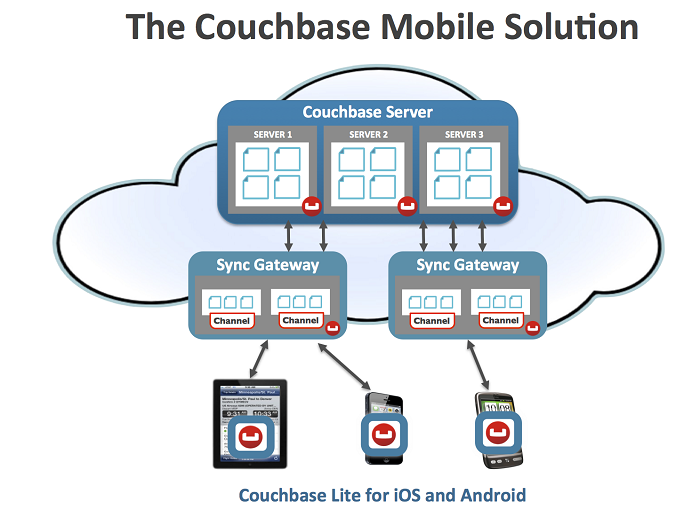
\includegraphics[height=0.25\textheight]{couchbase-lite}
\caption{Couchbase Lite and Sync Gateways. From \cite{couchbase-lite}}
\end{figure}

While traditional relational database management systems (RDBMS) are typically hard to scale out\footnote{also "Horizontal Scaling" - dividing a database over several servers after reaching the limit of upgrading a single server with more powerful hardware (vertical scaling)}, Couchbase offers a built-in distributed cache concept that can easily be scaled on more servers without modifying the application.

Queries are performed using the map reduce programming model originally developed by Google Engineers, allowing massive parallel execution (cf. \cite{MapReduceArticle}). This enables couchbase to perform computation and storage heavy big data analytics.

Couchbase was chosen for this work for it's mobile variant, it's synchronization abilities over several databases and it's JSON-based documents that are a good fit for the web back end and are easy to read and create manually.


\section{Typesafe Reactive Platform}

\subsection{Overview}

In 2013, Typesafe Inc. launched the "Reactive Manifesto", that was updated in September 2014 to the Version 2.0 \cite{reactivemanifesto}. The core message is as follows: "We believe that a coherent approach to systems architecture is needed, and we believe that all necessary aspects are already recognised individually: we want systems that are Responsive, Resilient, Elastic and Message Driven. We call these Reactive Systems."

The Typesafe Reactive Platform consists of the Play web framework, the Akka message driven runtime, the Activator build tool and of course the Scala programming language. It focuses on providing the tools needed to build highly responsive applications, that not only are easy to scale, but even able to increase and decrease the allocated resources at runtime to handle varying workload (thus be "elastic") and stay responsive even in case of failure (what is called to be "resilient").

Since it's publication, the manifesto and the platform gained rising attention. In my opinion, this platform has a high potential of getting the de facto standard for the development of how modern software systems, including web applications and web services, during the next years.

The Typesafe Reactive Platform is used in this thesis for building the back end part of the system, as Scala application with a Play web gui and an NoSQL Couchbase driver based on Akka, that will be introduced later. %TODO in Chapter xy

\subsection{Activator Tool}

Typesafe Activator is a dependency manager and build tool for the reactive platform built upon sbt (Simple Build Tool, sometimes Scala Build Tool). So it completely replaces sbt, understanding all commands formerly issued to sbt. In the Play framework, it replaces the Play command, which also was a wrapper around sbt. (cf. \cite{typesafeact}). It comes with an optional browser based ui for quickly creating some sample projects and an inspection feature for monitoring Play requests and akka actors. 

\subsection{Play Web Framework}


The Play Web Framework v1.0 was released on 19th October 2009. For version 2.0, released in March 2012, it was completely rewritten in Scala.
Although inspired by popular high-productivity web frameworks like Ruby on Rails or Groovy on Grails, it comes with full type safety typical for Scala but missed in the other frameworks.

Play is a full-stack web framework.

\begin{figure}[H]
\centering
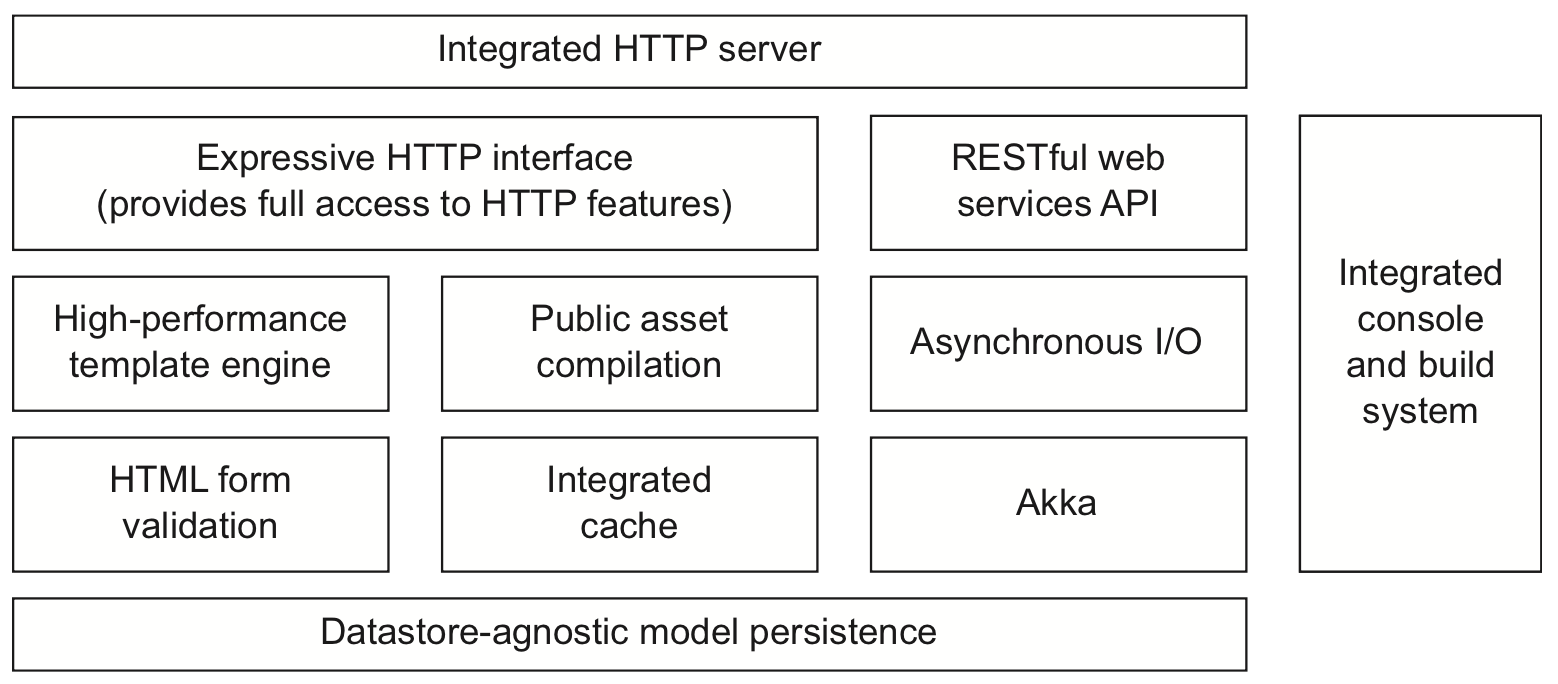
\includegraphics[height=0.25\textheight]{play-stack}
\caption{The Play framework stack. From \cite{play-book} with kind permission.}
\end{figure}

The key features that make Play a high-productivity web framework are:
 
\begin{itemize}
\item Integrated HTTP Server ("JBoss Netty")
\item RESTful web services API 
\item Type-safe templates for defining the html user interface
\item Central mapping from HTTP requests, including type-safe parameters, to the corresponding Scala controller method
\item Integrated build system that automatically rebuilds when the page is reloaded in the browser
\item Ability to test the web application without a browser or even a running web server and call controller methods or render templates directly from a Scala REPL with the pre-loaded project 
\item Support for AJAX, Comet and WebSockets
\item JSON mapping
%TODO
\end{itemize}

The Play framework is not the only Scala based web framework. According to Typesafe's CTO, they decided to integrate it in it's Platform instead of Lift or similar frameworks because it is completely written in Scala, uses Akka for asynchronous processing, providing a good concurrency handling, has the better type-safety even in html templates, and because it was the one with the greater momentum at the time the choice was made \cite[cf.][]{playdecision}.
